\documentclass[letterpaper]{article}
\usepackage{natbib,alifexi}
\usepackage[utf8]{inputenc}
\usepackage[english]{babel}
\usepackage{graphicx}
\usepackage{mathtools}
\usepackage{hyperref}
\usepackage{float}
\usepackage[colorinlistoftodos,prependcaption,textsize=tiny]{todonotes}


\title{Reinforcement learning approaches to movies recommendation}
\author{Antoine Carpentier$^{1}$, Pierre Gérard$^{2}$ \and Julian Schembri$^2$ \\
\mbox{}\\
$^1$Vrije Universiteit Brussel, Brussels \\
$^2$Université libre de Bruxelles, Brussels \\
antoine.carpentier@vub.ac.be, pierre.gerard@ulb.ac.be, julian.schembri@ulb.ac.be}


\begin{document}
\maketitle

\begin{abstract}
  The purpose of our research is to study reinforcement learning approaches to building a movie recommender system. We formulate the problem of interactive recommendation as a contextual multi-armed bandit, learning user preferences recommanding new movies and receiving their ratings. We show that using reinforcement learning solves the problem of exploitation-exploration tradeoff and the cold-start problem. We integrate the novelty of movies to the model. We explore a content based approach as well as a collaborative filtering approach and both yield viable recommendation results.
\end{abstract}

\section{Introduction}


Individuals sometimes have to settle on decisions without sufficient personal experience of the several choices. On a regular daily basis, their decisions depend on recommendations, advices and opinions from other individuals either by listening in conversations or by direct suggestion of movies, tv shows, holiday destinations, etc. Recommender systems help and enlarge this normal social process.

In a recommender system, individuals usually give behaviour information as data sources, which the system then use to learn users preferences in order to provide recommendation. The recommender's value lies in its capacity to make great matches between the recommenders and those looking for suggestions. Such systems are the strength of content providers such as Netflix \cite{netflix-article-recommender} and YouTube \footnote{http://www.youtube.com}, allowing them to make their content more attractive in order to increase views and to optimise the monetisation of their videos. It allows to infer the customer's center of interest and, if customers share some general behaviour, to detect improvements in content that can be made to better meet the expectations of the public. 


This work follows the steps of \cite{main} who have implemented a music recommendation system using reinforcement learning. In \cite{main}, they explain what could be done to adapt their work to movies recommandation and suggest to try a collaborative filtering approach. In our work, we first adapt their strategies to movies recommandation and then we try on some approaches they suggest.

The problem of movie recommandation is modeled as a contextual multi-armed bandit [\cite{sutton1998reinforcement}] [\cite{lu2010contextual}] which gives us the following advantages.

\begin{itemize}
	\item Learning incorporates user feedback (i.e. ratings of movies) into recommandations thus fitting diversity in users preferences, as opposed to \textit{context-free} multi-armed bandit,
	\item The model can take into account both a content based approaches and a collaborative filtering approaches,
	\item The model can use any type of features,
	\item Using a good policy balances exploration and exploitation thus mitigating the problems of cold-start and novelty.
\end{itemize}

The multi-armed bandit is a intensively studied reinforcement learning dilemma. It consists of a bandit (usually a casino slot machine) with $K$ arms, each giving a payoff $r$ sampled from an unknown probability distribution $p_{i}$. The player has a defined $n$ number of pulls and her goal is to choose wisely which arm to play in order to maximise the total payoff.

The contextual multi-armed bandit is a generalization of the multi-armed bandit where the reward obtained from each arm depends also on a \textit{context}. The context contains information about the arm and the player.


In the following sections, we will first introduce the methods used. Then we will review the results we obtained before discussing them.

\section{Methods}

\subsection{Data mining}

The data used is originated from IMDb \footnote{http://www.imdb.com/}. It is twofolds. The first part is a movie catalog containing relevant information about each movies such as the genre, keywords describing the content, the year, the mean rating and number of votes. That part is publicly available from IMDb FTP in a homemade format. The second part of data is RSS flux of movies watched and rated by IMDb users containing the title of the movie along with the rating and the time it was watched.

\subsection{Features extraction and selection}

The first challenge was to extract the features from the IMDb homemade format and convert it into a clearer \textit{csv} format.

In order to reduce the complexity of the algorithm, to focus on the learning matter and to avoid transforming the problem into a big data and parallelisation problem, a subset of movies and users was picked, counting up to about 430.000 user-movie pair. We picked the 1000 movies with the most votes and all users who have at least 50 ratings for those movies. This create a bias in the data, that we will need to evaluate in a future work based on full real-life data.

To keep the features vector simple, we selected only the genre and year for each movie. Those two features are categorical variable and in order to learn a single weight per feature (i.e. drama, crime, ..), a onehot encoding has been applied resulting in a blow up of the feature space to $n$ features, $n$ being the number of category.

\begin{table}[h]
\center{
\begin{tabular}{|c|c|c|c|c|}\hline
 Name       & Drama & Crime & Thriller & ... \\ \hline
Movie 1  & 0   & 0 & 1 & ...\\ \hline
Movie 2  & 1 & 1 & 1 & ...\\ \hline
Movie 3  & 0 &   0 & 0 & ...\\ \hline
... & ... & ... &  ...  &  ... \\ \hline
\end{tabular}
}
\vskip 0.25cm
\caption{Movies feature space}
\end{table}


\subsection{Dimension reduction}

The feature space resulting from the feature extraction process is quite large, making the recommendation computational intensive.
In order to deal with that problem, the feature space size has been reduced using Principal Components Analysis (PCA) [\cite{principalcompanalysis}].

The principal components analysis is a machine learning procedure that apply an orthogonal transformation to the dataset in order to obtain a new set of values that minimises the covariance. Those new variables are called principal components. There are ordered in term of variance, the first principal component having the highest variance and so on. When the procedure is applied a reduction to n-dimension consists of keeping the n-first principal components thus removing first the components with lesser variance.

For our dataset we kept the 20-first principal components out of about 50, keeping about 83\% of the variance of the original dataset.

\begin{figure}[H]
\begin{center}
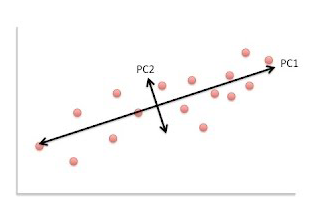
\includegraphics[width=2.1in]{img/pca.png}
\caption{Example of a 2 dimension PCA. A reduction to one dimension would keep only PC1.}
\label{pca}
\end{center}
\end{figure}

\subsection{Contextual multi-armed bandit modelling}

The movie recommendation problem can be seen as a contextual multi-armed bandit problem where each arm is a movie and a user can pull it (be recommanded to watch it). The context for each arm (movie) is a features vector containing the user features and the movie features. The reward (rating) obtained from pulling the arm (watching the movie) depends on this context. When the rating is returned, the user features are updated depending on the movie features and the rating.

This raises one concern : as the number of movies is gigantic, some movies might not be watched. To ensure that movies are not repeated too often, a \textit{novelty} parameter must be used.

\begin{figure}[H]
\begin{center}
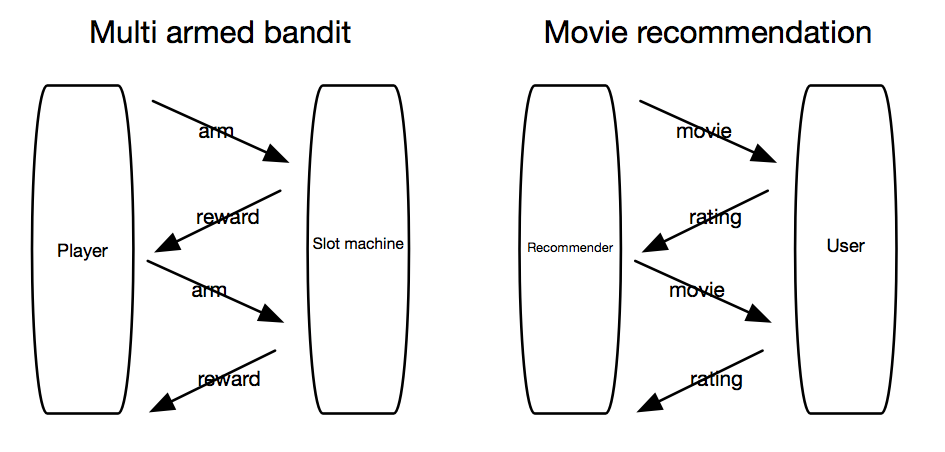
\includegraphics[width=3.4in]{img/schema.png}
\caption{Seeing a movie recommender as a contextual multi-armed bandit problem}
\label{schema}
\end{center}
\end{figure}

\subsubsection{Content based}

The content based model try to find a movie that is close to the learned user preferences $\boldsymbol{\theta}$. It takes into account the movie genre, movie year and novelty. Novelty can be defined as if the movie as been recently watched or not.

The movie genre and movie year can be considered as a onehot encoded vector $x$.
Without considering other factor, the utility of a user for a movie can be represented as the following.

\begin{center}
	$ \ U_{c} = \boldsymbol{\theta}^{T} \boldsymbol{x}$ 
\end{center}

Distinctive users have different preferences $\boldsymbol{\theta}$. Also, we do the hypothesis of a stationary true value for $\boldsymbol{\theta}$, meaning that while, we learn the user preference, its preferences stay the same.

The novelty is defined using the forgetting curve proposed by \cite{ebbinghaus1913memory} and defined as $ e^{\frac{t}{s}} $ with $t$ being the current time and $s$ an hyper-parameter defining how fast we forget and want a repetition. Obviously for movie an higher value of $s$ is needed compared to an $s$ that would be used for music. The utility for a user in term of novelty can be defined as follows.

\begin{center}
	$ \ U_{n} = 1 - e^{\frac{t}{s}} $ 
\end{center}

The combined utility or more explicitly the expected rating for a movie and a user is defined as follows.

\begin{center}
	$ \ U = \ U_{c} \times  U_{n} = (\boldsymbol{\theta}^{T} \boldsymbol{x}) \times (1 - e^{\frac{t}{s}}) $ 
\end{center}

The last task of the recommender is then to propose the movie with the highest expected rating to the user and update the user preferences $\boldsymbol{\theta}$ according to the difference in rating received and predicted.

\subsubsection{Collaborative filtering}

The collaborative filtering model try to find a movie that is a liked movie by a similar user. It takes into account others users rating and novelty of a movie.

The algorithm will start by finding a cluster of the user and $k$ others users by associating of the most similar user in clusters. The association is done by calculating the Pearson product-moment correlation coefficient on preferences $\boldsymbol{\theta}$ of the targeted user and others users. Then cluster users rating are considerate to be the utility of the user for those movie. In others words, similar user's movies rating become targeted user utility for those movies.

\begin{center}
	$ \ U_{f} = u $ 
\end{center}

Note that others users rating are weighted by the average means they give to movie to avoid biais.

The novelty if defined similarly as above, so the expected rating is :

\begin{center}
	$ \ U = \ U_{f} \times  U_{n} = u \times (1 - e^{\frac{t}{s}}) $ 
\end{center}



\subsection{Bandit strategies}

Many strategy to find an approximate solution have been developed over the years. A review of them is explain by \cite{kuleshov2014algorithms}.

\subsubsection{Random}

The random strategy is not a real strategy per se. It is a strategy where the player will only do exploration. It is mostly used as a basis to compare the effectiveness in term of reward or regret of an other algorithm.

\subsubsection{Greedy-epsilon}

The $\epsilon-greedy$ algorithm is widely used because it is fairly simple. For each round of the simulation, the algorithm selects the arm (movie) with the highest expected value based on the context vector with a probability of $1-\epsilon$ and selects a random arm with a probability $\epsilon$.

\subsubsection{Greedy time dependent}

The greedy time dependent is a variation of the previously mentioned greedy where $\epsilon$ variated over time in order to maximise the exploration at first and reduce it in order to increase exploitation over time.

\begin{center}
	$\epsilon = \frac{1}{\sqrt{t+1}}$
\end{center}

However, the effectiveness of variating $\epsilon$ over time is disputed by \cite{vermorel2005multi} whose did not find any practical advantage to using these method. As a result, we will test both approaches.

\subsubsection{Greedy UCB}

\todo{GreedyUCB}

\subsubsection{Exact Bayesian methods}

\todo{Bayesian methods}
% """Priors for the Bayesian models were set as uninformative ones or chosen based on preliminary simulation and user studies""" < ce qui notre tache très difficile

\subsubsection{Bayes inference}

\todo{Bayes inference}

\subsection{Simulation}

We conducted an empirical efficiency study of the algorithms mentioned above as well as the content based and collaborative filtering modelling. 

Experiments were conducted on personal computer and the programming language $python$ was used to implement models and algorithms.

The simulation consisted on simulating the interaction of a user and a recommender. Results can be found in section \ref{results} \todo{explain the simulation better}

\subsection{Metrics} \label{metrics}

In order to evaluate our algorithms and models in term of movie recommendation performance, an assortment of metrics retained. They could be formalised as follows.

\subsubsection{Cumulative regret}

For the $l$-th recommendation, the regret is defined as the difference between the maximum expected rating $ E[R^{l}] = max_{k=1...|S|} U_{k} $  and the expected rating $E[\hat R^{l}]$ of the recommended song is  $\Delta_{l} = E[\hat{R} ^{l}] - E[R^{l}]$. The cumulative regret for the $n$-th recommendation is then $ \sum_{l=1}^{n} \Delta_{l} = E[\hat{R} ^{l}] - E[R^{l}]$

\subsubsection{Accuracy (RMSE)}

The root-mean-square error is a frequently used measure of the difference between the predicted value and the actually observed value. In our case, the root-mean-square error will be the square of the difference between the expected value for the rating and the actual rating given by the user.

\subsubsection{Average rating}

The average rating is the simplest metric consisting of only the observed rating. It is interesting because it is a good indicator of how the user liked the recommendation.

\subsubsection{Computation time}

The last metric is the time needed to compute a recommendation. Indeed, usually a recommendation should be computed in a reasonable time, the system can't afford to make the user wait for several minutes before giving him a recommendation. However, one could argues that the computation could be parallelized on multi-core or on a big data cluster and.  \todo{dernier phrase in discussion}


% ------ results -------
\section{Results} \label{results}

This section will explore the different results obtained throughout all experiments made.

\subsection{Adaptation of \cite{main} to movie recommendation}

Here are the results of the adaptation of \cite{main} to movie recommendation using a greedy algorithm and the same content based model as described in that paper. Let's look at metrics defined in \ref{metrics}


\begin{figure}[H]
\begin{center}
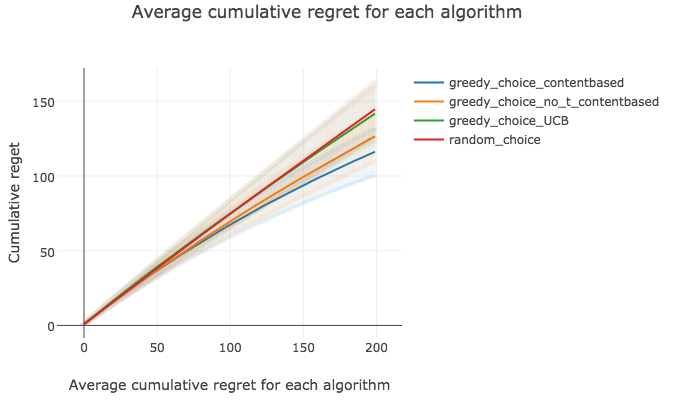
\includegraphics[width=0.47\textwidth]{img/greedy0.png}
\caption{capt0}
\label{greedy0}
\end{center}
\end{figure}

\begin{figure}[H]
\begin{center}
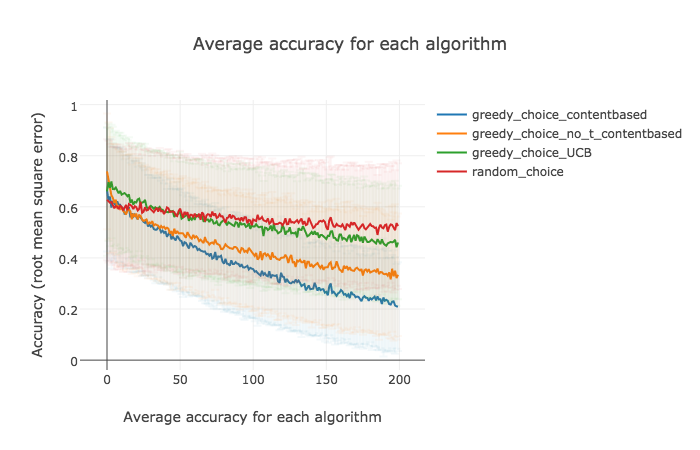
\includegraphics[width=0.47\textwidth]{img/greedy1.png}
\caption{capt1}
\label{greedy1}
\end{center}
\end{figure}

\begin{figure}[H]
\begin{center}
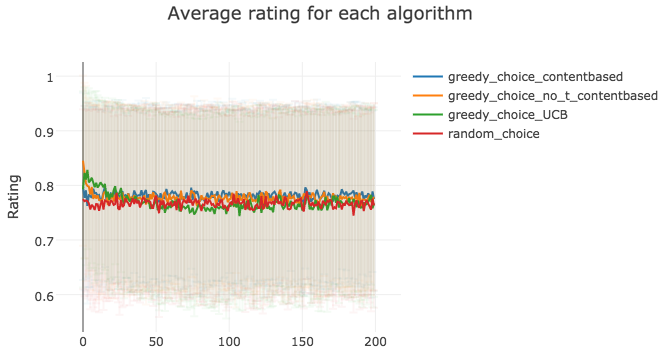
\includegraphics[width=0.47\textwidth]{img/greedy2.png}
\caption{capt2}
\label{schema2}
\end{center}
\end{figure}

\begin{figure}[H]
\begin{center}
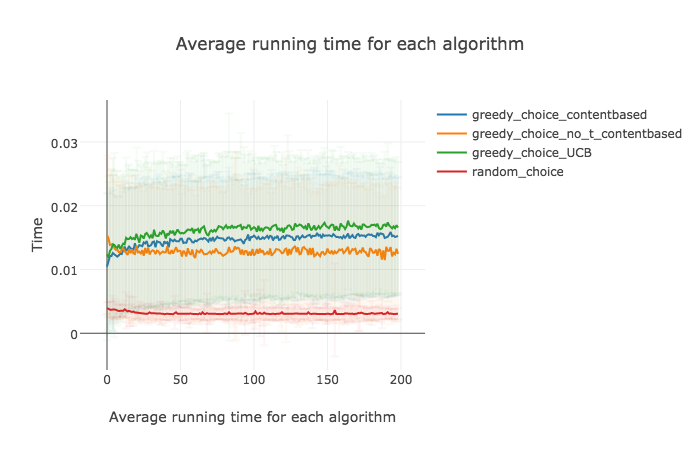
\includegraphics[width=0.47\textwidth]{img/greedy3.png}
\caption{capt3}
\label{greedy3}
\end{center}
\end{figure}


\subsection{Bayesian methods}

\todo{more diverse choice in bandit strategies including}


\subsection{Collaborative filtering and content based comparison}

\begin{figure}[H]
\begin{center}
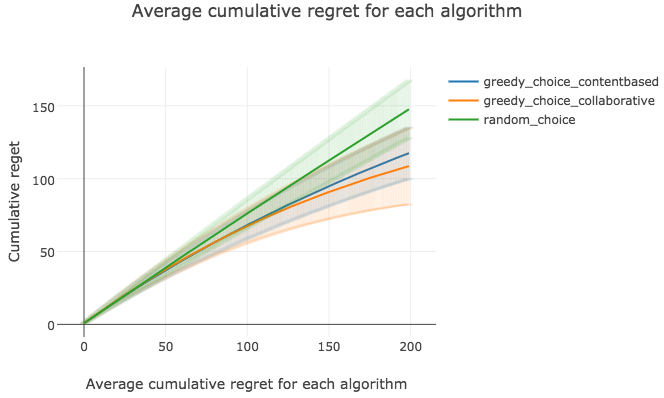
\includegraphics[width=0.47\textwidth]{img/collabo1.png}
\caption{Average regret}
\label{schema}
\end{center}
\end{figure}

\todo{result of collaborative filtering}

\subsection{Overall performance}

% ------ discussion -------
\section{Discussion}

\todo{would the result be correct recommendation, is it a viable way to do recommendation ? (expected result vs reality, time for a recommendation, accuracy, ....)}

\todo{which strategy to use and which not to use ( including why bayes-ucb is not viable (way too much time an requires a user study to bootstrap)}

\todo{content based vs collaborative, is collaborative viable}

\todo{maintenant qu'on a fait la recherche, si tu devais créer un vrai système tu utilises quoi comme technique}

\todo{futur work, what could be done if you give me 10 IA guys for a week}
% combined content based and collaborative filtering
% comparer avec une approche supervisé

\todo{futur work, real-life data, bias evaluation, big data toussa toussa}

\section{Conclusion}

blabla

\footnotesize
\bibliographystyle{apalike}
\bibliography{biblio}


\end{document}


%\begin{figure}[t]
%\begin{center}
%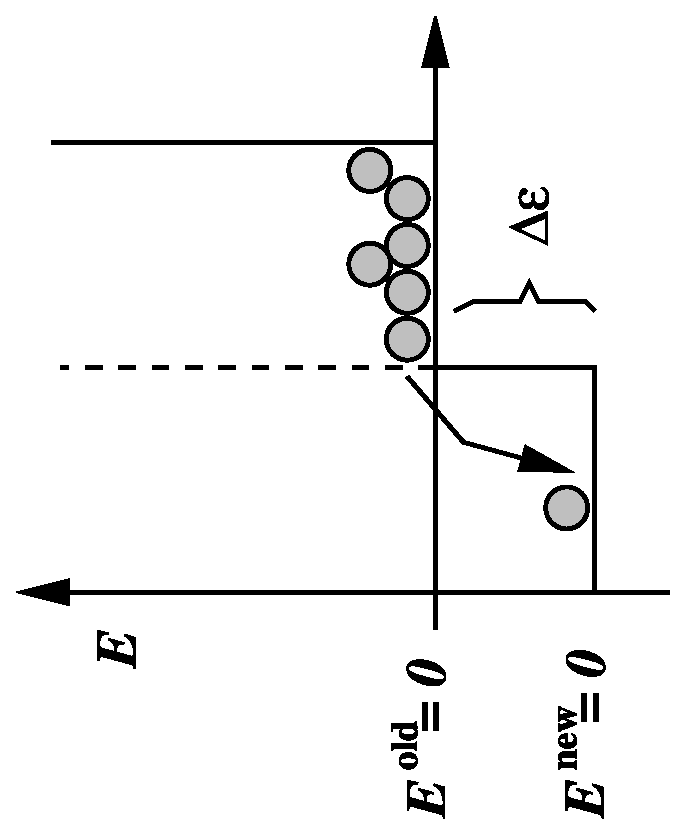
\includegraphics[width=2.1in,angle=-90]{img/fig1.eps}
%\caption{``Energies'' (inferiorities) of strings in a first-order
%  phase transition with latent heat $\Delta\epsilon$.}
%\label{fig1}
%\end{center}
%\end{figure}
